\chapter{模糊最大熵模型分类应用研究}

\section{iris数据集-鸢尾花分类}
\par
此数据是来自UCI的鸢尾花(iris)数据集.
这是一个经典的分类数据集,由Iris Setosa(山鸢尾)、Iris Versicolour(杂色鸢尾)和Iris Virginica(维吉尼亚鸢尾)三种不同类别的鸢尾花组成,
每个样本由四个属性组成,分别是Petal.Length(花瓣长度)、Petal.Width(花瓣宽度)、Sepal.Length(花萼长度)和Sepal.Width(花萼宽度).
按两两属性绘制原始数据如图\ref{散点图}.
\begin{figure}[!ht]
    \centering
    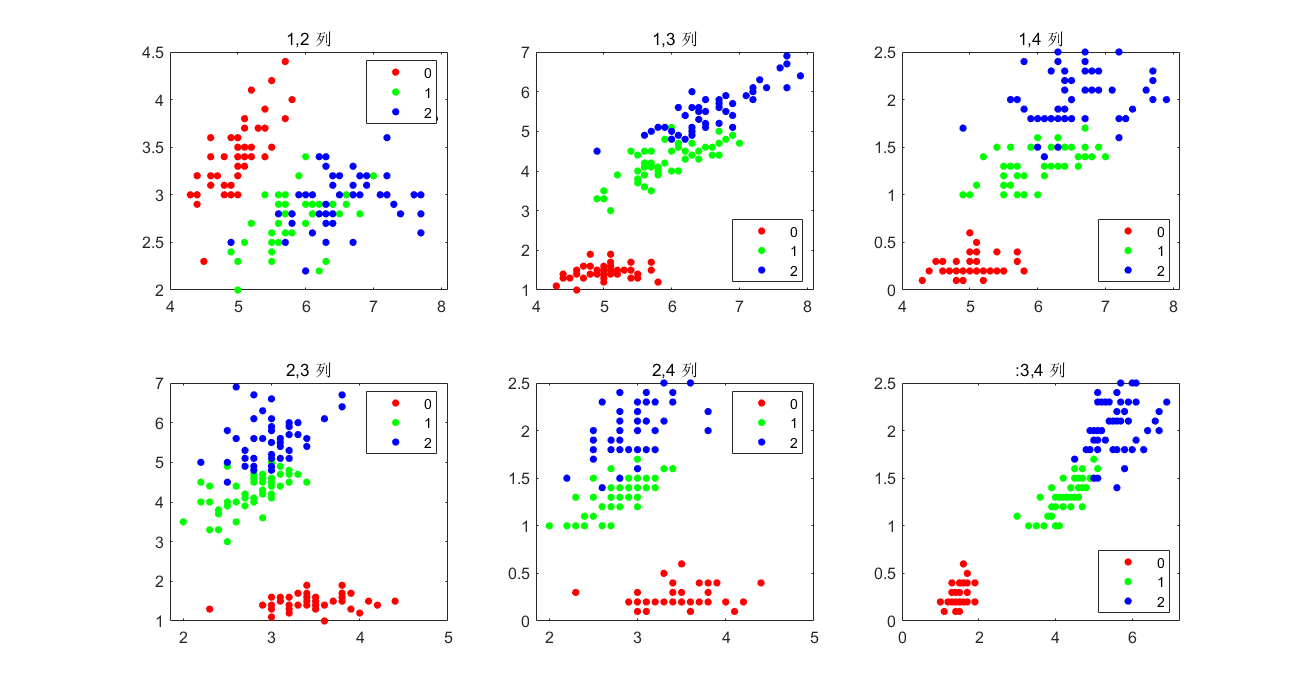
\includegraphics[scale=0.45]{sandiantu.png}
    \caption{原始数据散点图}
    \label{散点图}
\end{figure}
\par
0是山鸢尾,1是杂色鸢尾,2是维吉尼亚鸢尾.从图中可以看出,山鸢尾(红色)与其它两类可以较好地区分开来,杂色鸢尾与是维吉尼亚鸢尾则比较相近,不易区分.
\par 按4.1的算法对iris数据集进行聚类,结果如下:\\
\begin{table}[!ht]
    \label{iris聚类中心}
    \caption{iris聚类中心}
    \centering
    \begin{tabular}{c c c c c}
        \whline & sepal length & sepal width & petal length & petal width \\\whline
        $v_1$   & 5.0136       & 3.3903      & 1.5369       & 0.2781      \\
        $v_2$   & 6.4737       & 2.9437      & 5.1910       & 1.8012      \\
        $v_3$   & 6.0922       & 2.8186      & 4.6775       & 1.5731      \\
        \whline
    \end{tabular}
\end{table}
\newpage
\begin{figure}[!ht]
    \centering
    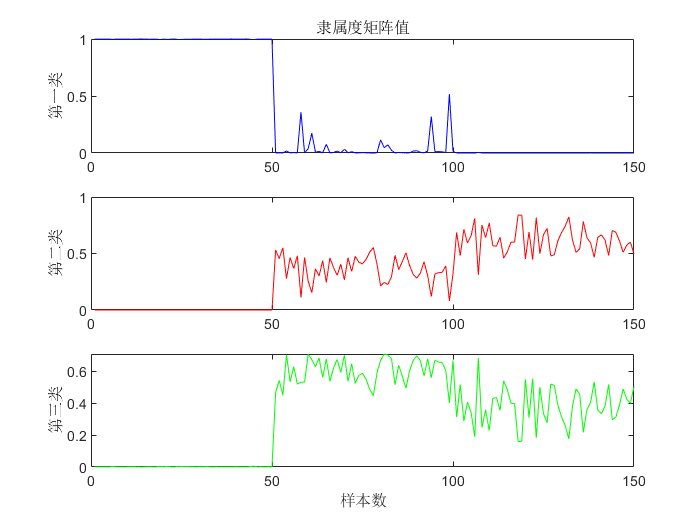
\includegraphics[scale=0.8]{lishudu.png}
    \caption{隶属度矩阵的值}
    \label{隶属度}
\end{figure}
从表\ref{iris算法比较}数据的比较中,我们可以看到,对于第一类,三个算法都做到了很好的识别,但是对于后两类非线性相关的类别,模糊最大熵模型比其他两个模型有着更好的表现.
\begin{table}[!ht]
    \label{准确率比较}
    \caption{准确率比较}
    \centering
    \begin{tabular}{c|c c c c}
        \whline 算法/各类准确率 & Setosa & Versicolour & Virginica & 总样本 \\\whline
        K-means                 & 100\%          & 96\%                  & 72\%                    & 89.4\% \\
        FCM                     & 100\%          & 76\%                  & 94\%                    & 90\%   \\
        MFE                     & 100\%          & 86\%                  & 98\%                    & 94.7\% \\
        \whline
    \end{tabular}
    \label{iris算法比较}
\end{table}

\newpage

\section{seeds数据集-种子分类}
seeds数据集是来自UCI的小麦种子,里面包括三种不同品种小麦的籽粒:Kama,Rosa和Canadian,每种70个元素,随机选择用于实验.
每个样本包括了面积、周长、紧凑度、籽粒长度、籽粒宽度、不对称系数和核槽的长度七个参数.我们选取前四个属性两两进行可视化如图\ref{seeds散点图}
\begin{figure}[!ht]
    \centering
    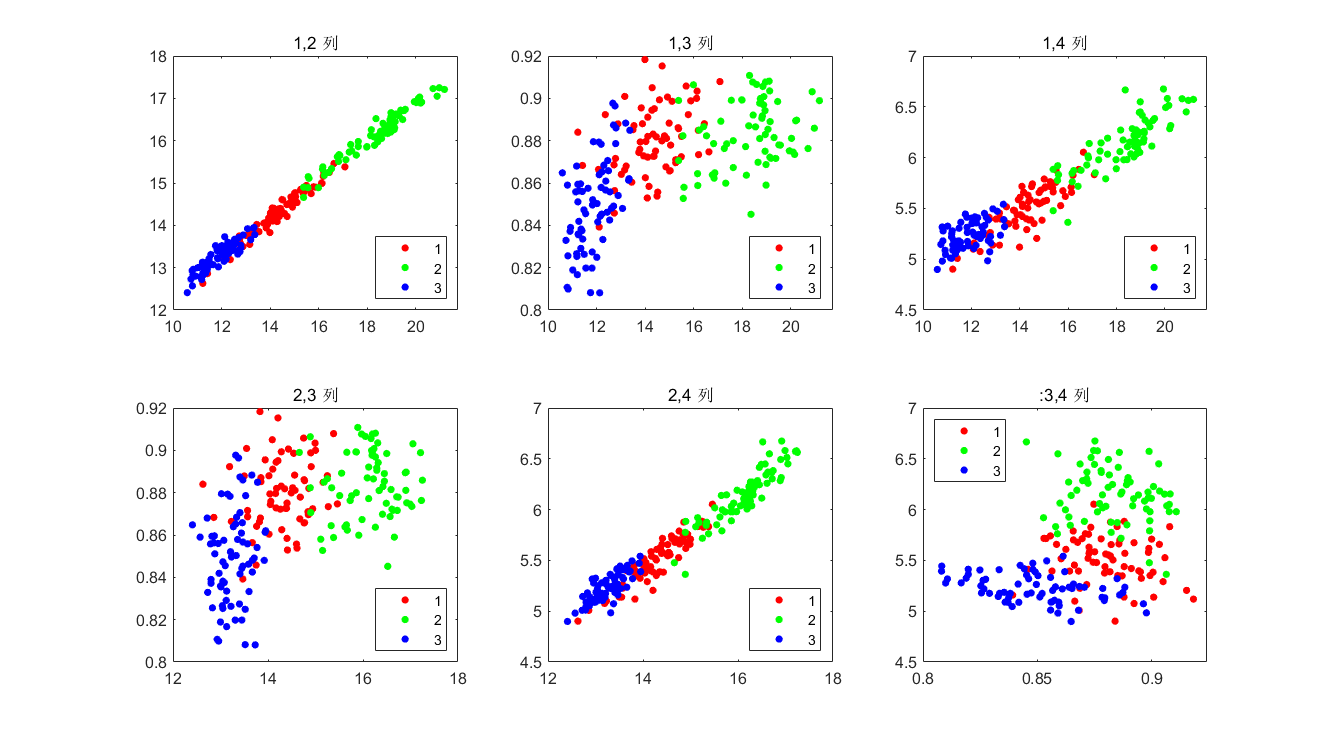
\includegraphics[scale=0.45]{seeds散点图.png}
    \caption{seeds数据集散点图}
    \label{seeds散点图}
\end{figure}
\par
聚类中心如表\ref{seeds聚类中心}:
\begin{table}[!ht]
    \label{seeds聚类中心}
    \caption{seeds聚类中心}
    \centering
    \begin{tabular}{c c c c c c c c}
        \whline & 面积    & 周长    & 紧凑度 & 籽粒长度 & 籽粒宽度 & 不对称系数 & 核槽的长度 \\\whline
        $v_1$   & 13.9310 & 14.1415 & 0.8721 & 5.4729   & 3.1682   & 3.1925     & 5.1668     \\
        $v_2$   & 18.3195 & 16.1181 & 0.8846 & 6.1446   & 3.6804   & 3.4856     & 5.9807     \\
        $v_3$   & 12.4027 & 13.4677 & 0.8567 & 5.2841   & 2.9409   & 4.4035     & 5.0930     \\
        \whline
    \end{tabular}
\end{table}
\par

\newpage
分类结果的隶属度矩阵:
\begin{figure}[!ht]
    \centering
    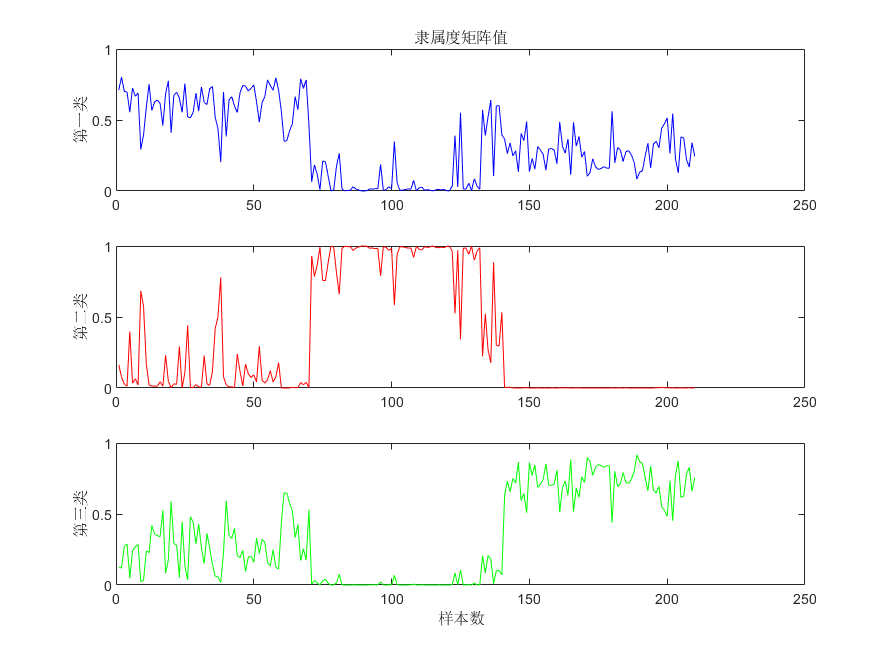
\includegraphics[scale=0.7]{seeds隶属度.png}
    \caption{seeds分类的隶属度矩阵的值}
    \label{seeds隶属度}
\end{figure}

\begin{table}[!ht]
    \label{seeds准确率比较}
    \caption{seeds分类准确率比较}
    \centering
    \begin{tabular}{c|c c c c}
        \whline 算法/各类准确率 & Kama  & Rosa & Canadian & 总样本 \\\whline
        K-means                 & 85.8\% & 85.8\% & 97.2\%     & 89.5\% \\
        FCM                     & 89.6\% & 85.8\% & 97.2\%     & 90.4\%   \\
        MFE                     & 87.3\% & 91.6\% & 96.8\%     & 91.5\% \\
        \whline
    \end{tabular}
    \label{seeds算法比较}
\end{table}
\section{结论}
    相比于Kmeans聚类,模糊最大熵模型对于非线性数据有更好的聚类效果,而相对于FCM聚类,由于增加了模糊最大熵的约束,
模糊最大熵模型将比FCM更快地收敛到局部最小值,即效率相对更高.